\documentclass[sigplan,10pt]{acmart}
\settopmatter{printfolios=true,printccs=false,printacmref=false}

\acmConference[Course paper, EDAN70]{Project in computer science}{Lund University}{Sweden}
\acmYear{\today}
\acmISBN{} % \acmISBN{978-x-xxxx-xxxx-x/YY/MM}
\acmDOI{} % \acmDOI{10.1145/nnnnnnn.nnnnnnn}
\startPage{1}

\setcopyright{none}

%% Bibliography style
\bibliographystyle{ACM-Reference-Format}
\usepackage{forest}
\usepackage{proof}
\usepackage{minted}
\usepackage{makecell}
\usepackage{changepage}
\usepackage{mathtools}
\usepackage{float}
\usepackage[section]{placeins}
\usepackage{caption}
\usepackage{graphicx}
\usepackage{subcaption}


\newcommand{\NL}[0]{ \hfill\\\noindent }
\newcommand{\coloneqtwo}{\mathbin{:\hspace{-0.5ex}\textsf{-}}}
\newcommand{\datalogM}{$\textit{Datalog}^M$}
\begin{document}

%% Title information5
\title[Short Title]{Datalog Implementation in JastAdd}         %% [Short Title] is optional;
                                        %% when present, will be used in
                                        %% header instead of Full Title.
%\subtitle{Subtitle}                     %% \subtitle is optional


%% Author information
%% Each author should be introduced by \author, followed by
%% \affiliation, and \email.

\author{Hampus Balldin}
\affiliation{
  \institution{C13, Lund University, Sweden}            %% \institution is required
}
\email{dat12hba@student.lu.se}          %% \email is recommended
\begin{abstract}
This paper presents the implementation of a new programming language belonging to the Datalog family.
A short background on Datalog, its theoretical foundations, and its applicability for practical problems is described.
A number of extensions to the core Datalog language are presented, the most novel of which is to allow predicates to be used as terms in atoms. As will be shown, this enables a compact description of various meta properties such as encoding what tables to output, or to give static types to predicates. 
\end{abstract}
\maketitle
\section{Introduction}
Datalog is a syntactically simple declarative language that allows the expression and evaluation of certain first-order logic propositions. From its' inception in the nineteen-eighties it received substantial interest from the academic community into the early nineteen-nineties\cite{Green:2013:DRQ:2688167.2688168}. The efforts primary drive were to enable knowledge based systems that allowed the generation of new facts based on rules stated using the logic programming paradigm. At the time, this had applications in both artificial intelligence as well as a complement to the traditional relational database querying systems such as SQL\cite{Ceri:1989:YAW:627272.627357}\cite{Bancilhon:1986:AIR:16894.16859}.

After a time of cooling interest, Datalog has emerged again as an attractive way to express complex inter-dependencies\cite{Green:2013:DRQ:2688167.2688168}. A notable example is from Program Analysis where frameworks such as Doop\cite{Smaragdakis:2010:UDF:2185923.2185939} make use of Datalog to derive e.g. call-graph and points-to information, both of which typically have mutually recursive dependencies in languages using dynamic dispatch. 

There are currently many Datalog implementations, some of which include Souffle\cite{Scholz:2016:FLP:2892208.2892226}, LogiQL\cite{Aref:2015:DIL:2723372.2742796}, Iris\cite{Bishop_iris-integrated}, and BDDBDDB\cite{Whaley:2005:UDB:2099708.2099719}. The implementations provide different evaluation methods and different extensions to the core Datalog language. This paper describes a common front-end that allows for source-to-source compilation. A common front-end enables a convenient way to compare the performance and expressive power of different Datalog implementations. An additional goal is to provide a library that can be used to implement and evaluate new inference schemes.

JastAdd \cite{Ekman:2007:JEJ:1297105.1297029} is a meta-compilation system that enables the expression of arbitrary graphs on top of an abstract syntax tree (AST). Information is propagated through the AST using so called Reference Attribute Grammars. JastAdd also supports aspects which allow the weaving of methods and class fields from different source locations into a single generated class. This enables easy extension of the generated AST classes with additional properties. In particular, it nicely permits the incremental addition of support for source-to-source compilation to different Datalog implementations. 

\subsection{Core Language}
There are many flavors of the Datalog language but they all build on a common core. 

%A \textit{program} $P$ consists of a set of \textit{Horn clauses} $H_1, \ldots H_n$. A horn clause has a \textit{head} and a \textit{body}. The head is a single \textit{atom} and the body is a sequence of atoms. A atom is identified by a \textit{predicate symbol} and a sequence of g\textit{terms}. An example of a propositional rule (without terms) is shown below:
\begin{align*}
A :- \;B_1, B_2, \ldots B_m
\end{align*}
\noindent
Above we have a single horn clause (hereafter called a \textit{rule}). It has head $A$ and body $B_1, B_2, \ldots B_m$. The intuitive meaning of the above rule is that if the conjunction of all the atoms in the body are true then we conclude $A$.

Datalog deals not only with propositional rules, but allows a restricted range of first-order propositions where each atom is associated with a sequence of terms. A term is either \textit{variable} or \textit{constant}. An atom that contain only constant terms is called a \textit{ground atom}. We further partition the predicates into extensional (EDB) and intensional (IDB). The EDB's are all predicates that are taken as input from an external database. The IDB's are the predicates that are not EDB and are intensionally defined through rules. The EDB's introduce \textit{facts}, i.e. ground atoms. One may additionally introduce facts by declaring a rule with a ground atom head that has an empty body. 

\begin{itemize}
\item The set of all constants in all facts is called the \textit{domain} and is denoted $\Omega$.
\item The set of all facts is called the \textit{active database instance} and is denoted $I$.
\end{itemize}
 
There are three main semantic interpretations of Datalog: model-, fixpoint-, and proof-theoretic semantics. \cite{Green:2013:DRQ:2688167.2688168}. A brief overview is given below.

\paragraph{Model-theoretic Semantics}\NL
A \textit{model} of a Datalog program $P$ is a consistent (satisfying all rules of $P$) extension of the initial EDB facts. Each rule is interpreted as a universally quantified rule. For example, below is given a rule and its' corresponding semantic interpretation. In the example $B(c_1, "C")$ is written as $(c_1, "C") \in B$ to emphasize the practical correspondence between predicates and relations.
\begin{align*}
A(x, y, "C") :- \;B_1(x, "C"), B_2("C", y), B_3(x, y)
\end{align*}
\begin{align*}
\infer{(c_1, c_2, "C") \in A}{%
	\forall c_1 \in \Omega.\;\forall c_2 \in \Omega. \;\; (c_1, "C") \in B_1, ("C", c_2) \in B_2, (c_1,c_2) \in B_3
}
\end{align*}
An inference algorithm attempts to find the \textit{minimal model}, i.e. a model $m$ of $P$ such that for any other model $m'$ of $P$, all facts of $m$ are in $m'$. In practice this means that an inference algorithm should only add a fact if it is required by the semantics of a rule (even if adding the fact may lead to an extended model of $P$). 

\paragraph{Fixpoint-theoretic Semantics}\NL
Begin with the set of all facts in the active database instance $I^0$. The set of new facts that can be derived (under model-theoretic semantics) using the rules of a program $P$ and the existing facts in $I^i$ is denoted $\Delta_i$. We get the following inductive definition of $I$:
\begin{align*}
&I^0 = \{ \text{EDB Facts in } P \}\\
&I^{i + 1} = I^i \cup \Delta_i 
\end{align*}
It can be shown(CITE) that the minimal model is computed as $I^{n}$ for $n$ such that $I^{n}$ = $I^{n + 1}$. Since $I^i \subseteq I^{i + 1}$ (monotonically increasing) and with the practical assumption of a finite domain, the fix-point algorithm is guaranteed to terminate.

\paragraph{Proof-theoretic Semantics}\NL
Consider a ground atom $A(C_1, \ldots, C_n)$. A query for the ground atom asks for a proof that $A(C_1, \ldots, C_n)$ is in the minimal model of a program $P$. A proof can be visualized as an \textit{and-or tree} $T$. $T$ has the proposition (ground atom) to prove as the root. At an OR-node, all possible rules are tested. If any of them succeed then the proposition has been proven. At an AND-node, all the child propositions need to be proven for the node to become true. An example is shown in figure \ref{figure:andOrTree}.
\begin{align*}
r_1: A :- \;B, C\\
r_2: A :- \;B, D
\end{align*}
\begin{figure}[ht!]
  \centering

\begin{forest}
for tree={circle, draw, l sep=1pt}
[A,blue 
	[$\lor$  
		[$\land$, edge label={node[midway,left] {$r_1$}}
			[B] 
			[C] 
		]
		[$\land$, edge label={node[midway,right] {$r_2$}}
			[B]
			[D]
		]
	]
]
\end{forest}
\caption{An and-or tree for rules $r_1: A :- \;B, C$, $r_2: A :- \;B, D$}
\label{figure:andOrTree}
\end{figure}
\noindent
When traversing the tree the model is updated with new facts that are needed to prove the root proposition. Those facts then become part of the extended model. 

\subsection{Security Features and Time Complexity}
Above a fact was stated to be a ground atom that is true in a given model. An axiomatic fact can be declared as a rule with no body: $A(t_1, \ldots, t_n)$. Datalog disallows axiomatic facts that contain variables. This is implied by the following more general rule: all variables occurring in the head of a rule must also occur in the body of the rule. This is called the \textit{range restriction property} \cite{Green:2013:DRQ:2688167.2688168}.

\subsection{Query Evaluation}



% Expression Problem
% (Knuth attribute Grammars)
% Parser / Lexer
% (How much is interesting to write here?)
\section{Core Language Implementation}
\newcommand{\sigmatwo}{\overline{\sigma}}
The current query evaluation mechanism for \datalogM is a bottom-up naive\cite{Green:2013:DRQ:2688167.2688168} evaluation. It is based on the fixpoint-theoretic semantics, deriving tuples from rules until no new tuples may be derived. The rule evaluation is performed using relational algebra (see e.g. \cite{Abiteboul:1995:FDL:551350}) and a thorough description is given in Appendix A.

\subsection{Mutual Dependencies and Predicate Ordering}
With multiple rules and potentially many mutual dependencies between the predicates, there is a need to find an order in which to apply the rules. Indeed, for mutually dependent predicates, all rules which may derive new facts for those predicates need to be iterated together. \textit{Stratification}\cite{Green:2013:DRQ:2688167.2688168} is the process of clustering the predicates that need to be computed together into so called \textit{strata} as well as to find an optimal order between the strata. The iterative fix-point algorithm is then run over each \textit{stratum} following the computed order. The process is formalized below.

A predicate $P_i$ \textit{directly depends} on predicate $P_j$ iff there exists a rule for which $P_i$ is in the head and $P_j$ is in the body. Let $Dep(P_i)$ be the set of predicates which $P_i$ directly depends on. The dependency graph $G_{DEP}$ has the set of predicate symbols as vertices and there is an edge from $P_i$ to $P_j$ iff $P_j \in DEP(P_i)$. A strongly connected component in $G_{DEP}$ then contains the predicates which are mutually recursive. Such a connected component can be found e.g. using Tarjan's algorithm \cite{Tarjan72depthfirst} and is called a stratum. By merging the vertices of $G_{DEP}$ into such strata we get a graph $G_{STRAT}$ with vertices being the strata of $G_{DEP}$ and edges the collapsed multi-edges from $G_{DEP}$. By construction there exists a total order on $G_{STRAT}$ with $S_1 < S_2$ iff $(S_1, S_2) \in Edge(G_{STRAT})$. The desired order is found by a reverse post-order search of $G_{STRAT}$.
\begin{figure*}[!hbt]
	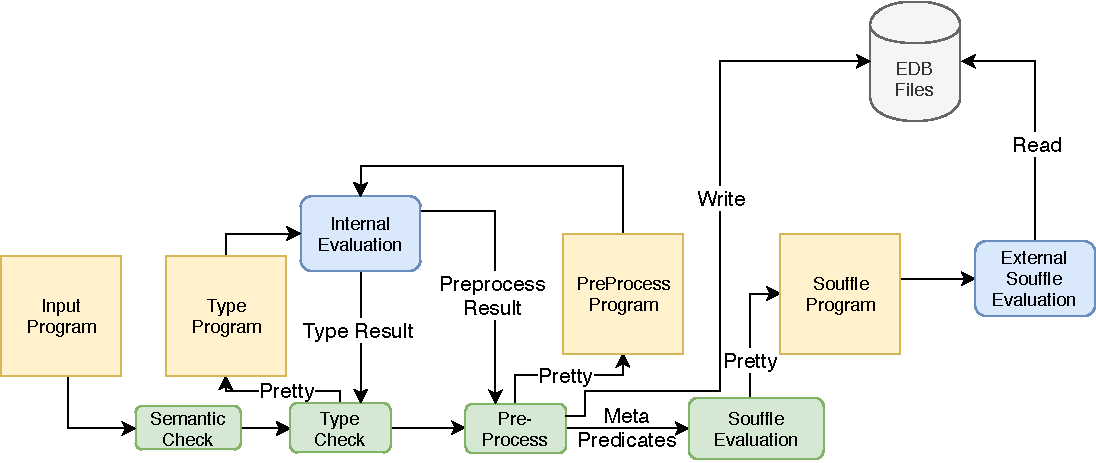
\includegraphics[scale=0.7]{img/souffleEval.pdf}
	\caption{Souffle Printing Pipeline. \textbf{Yellow}: A Datalog Program. \textbf{Blue}: An evaluation mechanism. \textbf{Green}: A compiler stage. }
	\label{figure:soufflePipeline}
\end{figure*}
\subsection{Cross Compilation}
In addition to internal evaluation, $Datalog^M$ supports cross-compilation, or pretty-printing, to Souffle\cite{SouffleHome}. The compilation pipeline is shown in figure \ref{figure:soufflePipeline}. First, a number of semantic checks are performed. For example, the semantic check ensures that all variables used in the head of a rule also occures in the body of the rule (the range restriction property\cite{Ceri:1989:YAW:627272.627357}). In the next stage, the program is type checked (type-checking is described in more detail in the following section). As was mentioned in the introduction (and will be explained in the next section), \datalogM supports meta-predicates. Souffle however has no such support so naturally it does not recognize the meta-semantics. To this end, a separate pre-process Datalog program is generated to evaluate all meta-predicates and subsequently output them as EDB files. Finally, the program is pretty-printed to a Souffle program $P_{Souffle}$. $P_{Souffle}$ declares the meta-predicates and loads them from the EDB files; the meta-predicates can then be used as ordinary predicates within the Souffle environment.
\section{Language Extensions}
A number of language features have been added in addition to the core Datalog features. Those extensions are listed and briefly described in the following subsections.
\vspace*{-5 pt}
\subsection{Negation}
A common datalog extension is to allow negation ($\neg$) of atoms. However, unrestricted negation introduces semantic issues as the following example illustrates:

\NL
{\centering
	$A(x) \coloneqtwo \neg B(x).\qquad\qquad[r_1]$ \NL
	$B(x) \coloneqtwo \neg A(x).\qquad\qquad[r_2]$\par
}

\NL
There are two issues with the above example. First, no unique minimal model exists: if $r_1$ is evaluated first then $A = \Omega, B = \emptyset$, and if $r_2$ is evaluated first then $A = \emptyset, B = \Omega$. Second, even if a unique minimal model exists, guaranteed termination is lost since negation removes monotonicity (adding tuples to one relation may remove tuples from another). The first issue is addressed by ensuring that all variable terms used in a negated atom are also used in a non-negated (\textit{positive}) atom. Second, we require that each stratum retains the monotonic property, in particular this means that mutual recursive dependencies must be positive.

With the above restrictions, negation becomes a filtering rule; an occurrence of a negated atom within a rule has already been fully evaluated when that rule is considered in a stratum. Thus restricted negation can be implemented as a set-difference over the artificial body relation (introduced in the previous section).

\subsection{Built-in Predicates and Expressions}
Most (if not all) Datalog systems include various built-in predicates for discarding certain results based on some criteria. The current implementation includes the usual binary predicates $=, \neq, \leq, \ldots$ They can be used with expressions over the usual binary operators $+,-,*,/$. To continue with the order example, a relation that picks ordered tuples with elements at least two units apart is shown below:

\NL
{\centering
	$TwoGapOrder(x, y) \coloneqtwo Order(x, y), x \leq y - 2.$ \NL
}

\vspace*{-\baselineskip}
\subsection{Object Creation}
A special bind predicate was introduced to allow for the creation of new objects. Combined with \textit{aggregates}, such as counting the number of elements in a relation, this is a useful way to let datalog reason about properties of the currently evaluating program. However, the new expressive power may lead to non-terminating programs as the following example for generating the natural numbers illustrates. No checks have been added to detect this divergence.

\begin{minted}{yaml}
Nat(0).
Nat(y) :- Nat(x), BIND(y, x + 1).
\end{minted}
\noindent

\subsection{Type System}
The language includes a simple type system. The basic types are:
\begin{align*}
	String : * \quad Integer : *, \quad PredRef : * 
\end{align*}
\noindent
The types are themselves terms and the star means the type of a type. The $PredRef$ type is used to reference predicates and forms the basis for meta-predicates. Last, the type system has a List \textit{type-constructor}, i.e. it is a function from a term of type $*$ that gives another term of type $*$:
\begin{align*}
	List : * \rightarrow *
\end{align*}
\noindent
The types are introduced through a special type predicate:
\begin{align*}
	TYPEOF : PredRef \times List(*)
\end{align*}
In this way, $TYPEOF$ relates the referenced predicate with a list of types:
\begin{align*}
TYPEOF('A, [t_1, \ldots, t_n]). &\implies A : t_1 \times \ldots \times t_n\\
\end{align*}
\vspace*{-\baselineskip}\vspace*{-\baselineskip}\vspace*{-\baselineskip}
\subsubsection{Type Checking and Type Inference}
Type-checking and left-to-right type inference of a Datalog program $P$ is done through the generation of another datalog program $P_T$. The type checking is performed in three passes. First $P_T$ is generated from $P$. Second, the evaluation of $P_T$ gives the local type information for the terms in each rule. Third, global consistency is checked over the local result. The process is perhaps best illustrated with an example. Consider the source program $P$ in figure \ref{figure:sourceP}. The transformed type program $P_T$ is shown in figure \ref{figure:sourcePT}.
\begin{figure}[!ht]
\begin{minted}{yaml}
TYPEOF('A, [String Integer]).
B(1, 2).
C(x, y, z) :- A(x, y), B(z, z).
D(x, y, z) :- B(x, y), A(z, y).
\end{minted}
\caption{The source program $P$.}
\label{figure:sourceP}
\end{figure}

\begin{figure}[!ht]
\begin{minted}{yaml}
A(String, Integer), B(Integer, Integer).
Typeof(PredRef, List(Type)).
C(x, y, z)     :- A(x, y), B(z, z).
D(x, y, z)     :- B(x, y), A(z, y).
Rule0(x, y, z) :- C(x, y, z), A(x, y), B(z, z).
Rule1(x, y, z) :- D(x, y, z), B(x, y), A(z, y).
\end{minted}
\caption{The transformed type program $P_T$.}
\label{figure:sourcePT}
\end{figure}
\noindent
A new rule predicate $r^{'}_i$ is added to $P_T$ for each rule $r_i$ in $P$. The head of $r^{'}_i$ is given a unique name (in the example $Rule0$, $Rule1$) and has as terms all the variables occurring in $r_i$. The body of $r^{'}_i$ consists of all the atoms in $r_i$. Additionally, the initial type facts are added. This gives the basis for local type-checking. To provide left-to-right type inference, the rules in $P$ are added to $P_T$ as-is. In the example, this allows the derivation of the types for $C$, and $D$. 
The example has a single solution for the rule types:
\begin{align*}
Rule0 : String  \times Integer \times Integer\\
Rule1 : Integer \times Integer \times String
\end{align*}
The rule-type solution gives the \textit{type-environment} $\Gamma$ in which the rule is executed: $\Gamma : Rule \rightarrow Variable \rightarrow *$. Using $\Gamma$, a global pass can trivially check that the type of each atom is unique across all rules.

\subsection{Meta-Predicates}
The language needs a way for the user to communicate certain properties about the datalog-program $P$ to the interpreter $I$.
An example of such a property is what relations to load as EDBs.
In turn, $I$ makes certain information available to $P$ which allows $P$ to make inference on properties of itself.
The information passing is done through a collection of pre-defined atoms. The currently supported such meta-predicates are listed in figure \ref{figure:metaatoms}. As is shown in the table, $EDB$ and $OUTPUT$ pass information from $P$ to $I$, $ATOM$, and $PRED$ pass information from $I$ to $P$. $TYPEOF$ initially provides $I$ with information about the given types. After successful type-checks and possibly type-inference, $I$ makes the result available to $P$, again through $TYPEOF$. In this way, $TYPEOF$ is a bi-directional predicate. Figures \ref{figure:outputatom}, \ref{figure:edb} show two examples of possible usages for the meta-predicates.

\begin{figure}[!ht]
	\begin{adjustwidth}{-0.5cm}{}
\begin{tabular}{ | c | c | c | }
	\hline
    \textbf{Predicate}  & \textbf{ Type } & \textbf{Semantics}\\
	\hline
    \multicolumn{3}{|c|}{\textbf{Datalog Program $\rightarrow$ Interpreter}}\\
    % \multicolumn{3}{|c|}{}\\
	\hline
	$EDB$  & $PredRef \times String$ & \makecell{$('A, s) \in EDB$ \\ Tuples in file $s$ loaded into $A$} \\
	\hline
	$OUTPUT$ & $PredRef$ & \makecell{$('A) \in OUTPUT$ \\ Tuples in $A$ printed to ''$A$.csv''} \\
	\hline
    \multicolumn{3}{|c|}{\textbf{Datalog Program $\leftarrow$ Interpreter}}\\
    % \multicolumn{3}{|c|}{}\\
	\hline 
	$ATOM$ & $PredRef$ & \makecell{$('A) \in ATOM$\\ $A$ is a user-defined atom.} \\
	\hline
	$PRED$ & $PredRef$ & \makecell{$('A) \in PRED$\\ $A$ is any occurring atom.} \\
	\hline 
    \multicolumn{3}{|c|}{\textbf{Datalog Program $\leftrightarrow$ Interpreter}}\\
    % \multicolumn{3}{|c|}{}\\
	\hline 
    $TYPEOF$ & $PredRef \times List(*)$ & \makecell{$('A, [t_1,\ldots, t_n]) \in TYPEOF$\\ $A : t_1 \times \ldots \times t_n$.} \\
	\hline
\end{tabular}
\end{adjustwidth}
\caption{A list of supported meta-predicates. The semantics column shows an if-and-only-if relation between the upper and lower statements.}
\label{figure:metaatoms}
\end{figure}

\begin{figure}[!ht]
\begin{minipage}{4cm}
\begin{minted}{yaml}
OUTPUT('OUTPUT).
OUTPUT(x) :- ATOM(x). 
\end{minted}
\end{minipage}
\vspace*{-10pt}
\caption{Printout all user defined-atoms as well as the $OUTPUT$-relation.}
\label{figure:outputatom}
\end{figure}

\vspace*{-\baselineskip}
\begin{figure}[!ht]
\begin{minipage}{4cm}
\begin{minted}{yaml}
EDB('EDB, "EDB.csv"). 
\end{minted}
\end{minipage}
\vspace*{-10pt}
\caption{Load the tuples that describe what to load as EDB files from the external database file EDB.csv}
\label{figure:edb}
\end{figure}

\vspace*{-15pt}
\section{Evaluation}
\subsection{Correctness}
\subsection{Performance}
\subsection{Expressive Power}

\vspace*{-5pt}
\section{Related work}
\subsection{Souffle}
Souffle implements a semi-naive evaluation\cite{Green:2013:DRQ:2688167.2688168} and performs a range of different optimizations before emitting highly templated C++ code\cite{Scholz:2016:FLP:2892208.2892226}. It focuses on performance and is for example used in program analysis\cite{Smaragdakis:2010:UDF:2185923.2185939}. It does not provide meta-predicates but instead uses special directives to declare what files should be used as EDBs, what relations should be printed, and what the type of a predicate is. It does however provide a number of built-in functions and aggregates that are not supported by $Datalog^M$\cite{SouffleHome}.

\vspace*{-8pt}
\subsection{Other}
IRIS \cite{Bishop_iris-integrated}\cite{IrisGithub} is an Open Source Datalog implementation written in Java. IRIS supports bottom-up evaluation strategies (both naive and semi-naive), as well as top-down (proof-theoretic semantics) strategies\cite{IrisGithub}. It was developed primarily as a research-tool for Semantic Web-related technologies and supports XML Schema data types.\cite{XMLDataType}.

BDDBDDB\cite{Whaley:2005:UDB:2099708.2099719} was developed at Stanford in the early 2000s and used the then novel technique to store relations as so called binary-decision diagrams (BDDs). BDDs encode relations as binary functions represented as directed acyclic graphs. The encoding allows compression of the relations and can be very memory efficient. Memory efficiency is important in e.g. program analysis, which is the main use-case that the project targeted\cite{Whaley:2005:UDB:2099708.2099719}.
\section{Conclusion}
This paper describes a working Datalog implementation with a number of extensions to the core Datalog semantics. In particular, the addition of predicate references in conjunction with a number of meta-predicates permit compact descriptions of Datalog programs. Together with cross-compilation to another more efficient Datalog implementation such as Souffle, \datalogM has the potential to grow into a useful Meta-Compilation system for specifying Datalog programs. Even so, performance is one area where \datalogM is currently lacking. The evaluation shows that two optimizations in particular would be worthwhile; implementing Semi-naive evaluation, and to add relation indexing in order to decrease the time-complexity of the \textit{join}-operation.
%The JastAdd system
\begin{acks}
Thank you Christoph Reichenbach for your many insights and helpful guidance throughout this project.
\end{acks}
\bibliography{bibl}
\clearpage
\section{Appendix A: Relational Algebra for Rule Evaluation}
Consider the following example:
\begin{align*}
&Order(1, 2),\; Order(2, 3). \quad\quad\quad\quad\quad\quad\quad\quad\quad[r_1]\\
&Order(x, z) \coloneqtwo Order(x, y),\; Order(y, z). \;\quad\quad\quad[r_2]
\end{align*}
\noindent
Rule $[r_1]$ states that the orders $1, 2$ and $2, 3$ holds. Rule $[r_2]$ states that the binary $Order$ relation is transitive. The BUN evaluation proceeds as follows. For each rule that is evaluated, an artificial body-relation $B$ is introduced. The body-relation will be incrementally populated and extended through the evaluation of the atoms in the body. 

Initially, the relation associated with each atom is unnamed, i.e. the columns of the relation have no name-restrictions. Given a rule $r$, we order the atoms from the body of the rule as $A_1, \ldots, A_n$. We will consider each atom in turn and use the body relation $B$ as an accumulator. The equations describing the rule-evaluation process is as follows (the notation is explained below):
\begin{align*}
B^{0} &\leftarrow \top \\
B^{i + 1} &\leftarrow B^{i} \bowtie \sigmatwo_{Term(A_{i + 1})}\;(A_{i + 1}), \; i = 0, \ldots, n - 1\\
H & \leftarrow H \cup \Pi_{Term(H)}(B^n)
\end{align*}
\noindent
The body relation is initially assigned to $\top$ denoting an unknown relation: $\top \bowtie R = R \bowtie \top = R$. The $Term$ function gives the terms in the given atom. $H$ is the head of rule $r$. A selection is then done for the atom. The special selection operator is denoted $\sigmatwo$. Informally it selects a set of tuples from the relation associated with the atom that satisfies the constraints imposed by the terms of the atom. As a more formal example:
\begin{align*}
\sigmatwo_{x,x,y,c} = \rho_{x/x_1, y/y_1} \circ \Pi_{x_1, y_1} \circ \sigma_{x_1 = x_2, C_1 = c} \circ \rho_{x_1/N_0, x_2/N_1, y_1/N_2, C_1/N_3}
\end{align*}

The selection is for three variables $x, x, y$ and a constant $c$. First the rename operator $\rho$ is used to rename the columns of the relation ($N_i$ is an artificial initial name for column $i$). Then the ordinary $\sigma$ operator selects all tuples such that the corresponding variables and constants match under the given naming. The result of the selection is then projected (discarding duplicates and constants) using the projection operator $\Pi$, and finally the inverse renaming is performed.

The selection result is joined ($\bowtie$) with the current body relation $B^{i}$ to form the next body relation $B^{i + 1}$. In our example (assuming that $r_1$ has been evaluated) we get:
\begin{align*}
B^{1} &\leftarrow \sigmatwo_{x, y}\;(Order) = \{(1, 2), (2, 3)\}_{x, y}\\
B^{2} &\leftarrow B^{1} \bowtie (\sigmatwo_{y, z}\;(Order) = \{(1, 2), (2, 3)\}_{y, z})\\
      &= \{(1, 2), (2, 3)\}_{x, y} \bowtie \{(1, 2), (2, 3)\}_{y, z}\\
      &= \{(1,2,3)\}_{x,y,z}
\end{align*}
\noindent
Finally we project the result of $B^n$ and add the new tuples to the head relation:
\begin{align*}
Order & \leftarrow Order \cup (\Pi_{x,z}(\{(1,2,3)\}_{x,y,z}) = \{(1,3)\})
\end{align*}
\noindent
The process is iterated until a fix-point is found, i.e. until no new tuples can be derived from the set of rules. In our example, iterating $[r_2]$ again gives no new tuples and so the $Order$ relation has been computed as: $\{(1,2), (1,3), (2,3) \}$.
\clearpage
\section{Appendix B: Correctness of Type Algorithm}
For an atom $A$ in the type algorithm, let the corresponding set of tuples be denoted $A_R$. The typing algorithm reports a type error in one of two cases:
\begin{align*}
&\exists A \in PRED_{P_T}.\;\;|A_R| > 1 \quad\quad (1)\\
&\exists A \in PRED_{P_T}.\;\;|A_R| = 0 \quad\quad (2)
\end{align*}
\noindent
A Datalog program $P$ is said to be \textit{well-typed} if:
\begin{align*}
\forall A \in PRED_{P_T}. \;\; |A_R| = 1 \quad\quad (3)
\end{align*}
\noindent
Let $Pos(x, A)$ give the coordinate of term $x$ in predicate $A$, and $A[n]$ give type of $A$ at coordinate $n$. A rule with two atoms using the same variable name gives a \textit{type constraint}:
\begin{align*}
\infer[(\textit{C-VarLeft})]{A[Pos(x, A)] = \tau}{\begin{array}{c c} &B[Pos(x, B)] = \tau\\&\exists Rule: \ldots, A( \ldots, x, \ldots), \ldots, B(\ldots, x, \ldots), \ldots\end{array}}
\end{align*}
\begin{align*}
\infer[(\textit{C-VarRight})]{B[Pos(x, B)] = \tau}{\begin{array}{c c} &A[Pos(x, A)] = \tau\\&\exists Rule: \ldots, A( \ldots, x, \ldots), \ldots, B(\ldots, x, \ldots), \ldots\end{array}}
\end{align*}
\noindent
Let the type of a constant term $t$ be given by $T(t)$. We get the following constraint for constants:
\begin{align*}
\infer[(\textit{C-Constant})]{A[Pos(t, A)] = T(t)}{\exists Clause\;C: \ldots A(\ldots, t, \ldots), \ldots, \;\; t : Constant } 
\end{align*}
\noindent
Finally, the semantics of $TYPEOF$ is added as a rule:
\begin{align*}
\infer[(\textit{C-TypeOf})]{A[Pos(\tau, TYPEOF)] = \tau}{\exists Fact: \; TYPEOF('A,\ldots, \tau, \ldots) } 
\end{align*}

\noindent
We say that a type algorithm is \textit{correct} if the type solution satisfies the listed constraints together with the additional requirement that in a valid type assignment, each predicate is assigned exactly one type (property (3) above). \textit{C-TypeOf} is satisfied by the type-checking algorithm by construction. We now show that it additionally satisfies \textit{C-Constant} and \textit{C-Var}. Together with properties (1), (2) this is enough to show correctness since $(3) \iff \neg ((1) \lor (2))$.

\paragraph{Proposition: } \textit{The type-checking algorithm satisfies C-Constant}\NL
A clause is either a fact or a rule. All facts are lifted to the type level and thus trivially satisfy \textit{C-Constant}. Thus assume that have a rule with a constant use in an atom A. We will get a corresponding type-rule with head $R_i$ with $A$ unconditionally in the body:
\begin{align*}
R_i(\ldots) \coloneqtwo \ldots A(\ldots, c, \ldots) \ldots
\end{align*}
By the Datalog semantics, $|R_i| > 0$ if can derive that A contains a fact with the constant (lifted type) $c$ at coordinate $Pos(c, A)$. Since there is no other clause that derives facts for $R_i$, this is the only way to satisfy $|R_i| = 1$ (if $|R_i| \neq 1$ then algorithm fails due to (1), (2)).\\\hspace*{200pt}$\blacksquare$

\paragraph{Proposition: } \textit{The type-checking algorithm satisfies C-Var*}\NL
Since C-VarLeft and C-VarRight are completely symmetrical it suffices to show for C-VarLeft.
Assume that we have a rule $R$ that gets transformed to a type-rule with head $R_i$:
\begin{align*}
&R_i(\ldots, x, \ldots) \coloneqtwo \ldots, A( \ldots, x, \ldots), \ldots, B(\ldots, x, \ldots), \ldots\\
&B[Pos(x, B)] = \tau
\end{align*}
\noindent
The algorithm reports a type error iff (3) does not hold for the type-program. Thus $B[Pos(x, B)]$ has $\tau$ as the only member.
By the Datalog semantics (and from the fact that no other rule populates $R_i$), (3) holds if and only if $A[Pos(x, A)] = \tau$. \\\hspace*{200pt}$\blacksquare$
\clearpage
%\section{Appendix C: Plots for Experimental Data}
%\begin{figure}[!htb]
%%	\hspace*{-25pt}
%%	\begin{minipage}[b]{.5\textwidth}
%		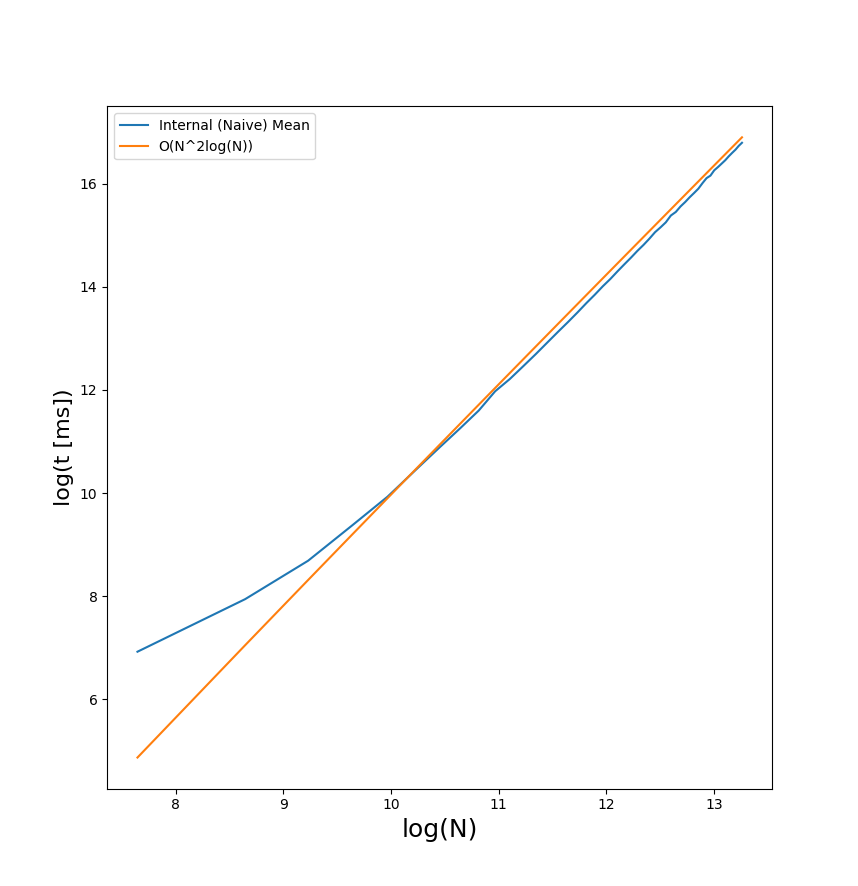
\includegraphics[width=0.9\linewidth]{img/internalloglog.png}
%	%\end{minipage}%
%%	\hspace*{-40pt}
%%	\begin{minipage}[b]{.5\textwidth}
%%		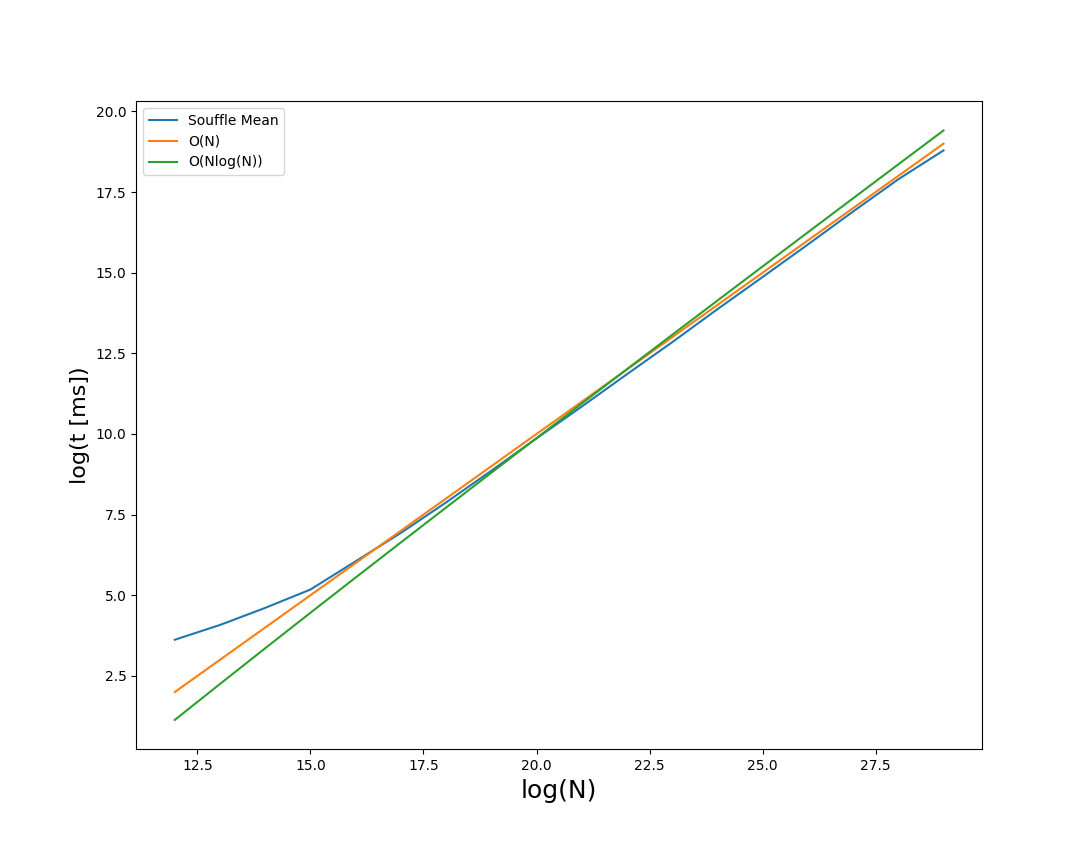
\includegraphics[scale=0.35]{img/souffleloglog.png}
%%	\end{minipage}
%%	\label{figure:natExperimental}
%	\caption{Nat Example, Internal Evaluation (Naive)}
%\end{figure}
%\begin{figure}[!htb]
%	\centering
%	%	\hspace*{-25pt}
%	%	\begin{minipage}[b]{.5\textwidth}
%	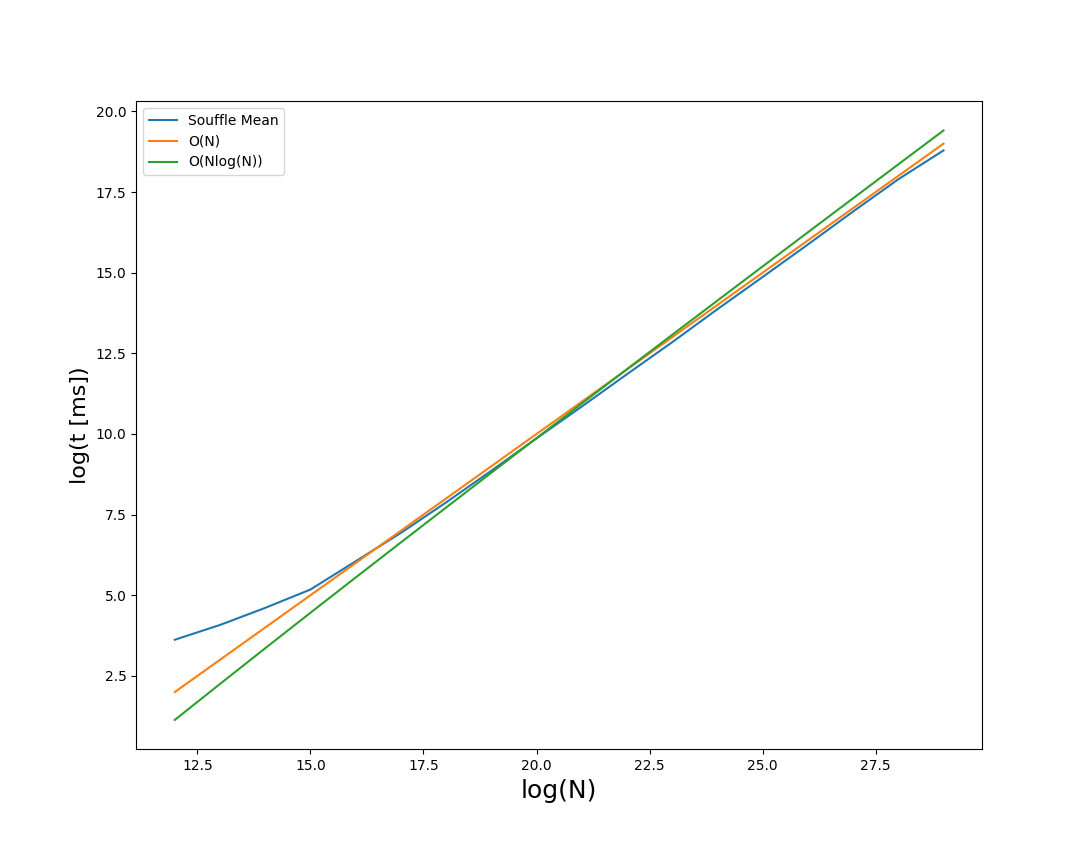
\includegraphics[width=1.0\linewidth]{img/souffleloglog.png}
%	%\end{minipage}%
%	%	\hspace*{-40pt}
%	%	\begin{minipage}[b]{.5\textwidth}
%	%		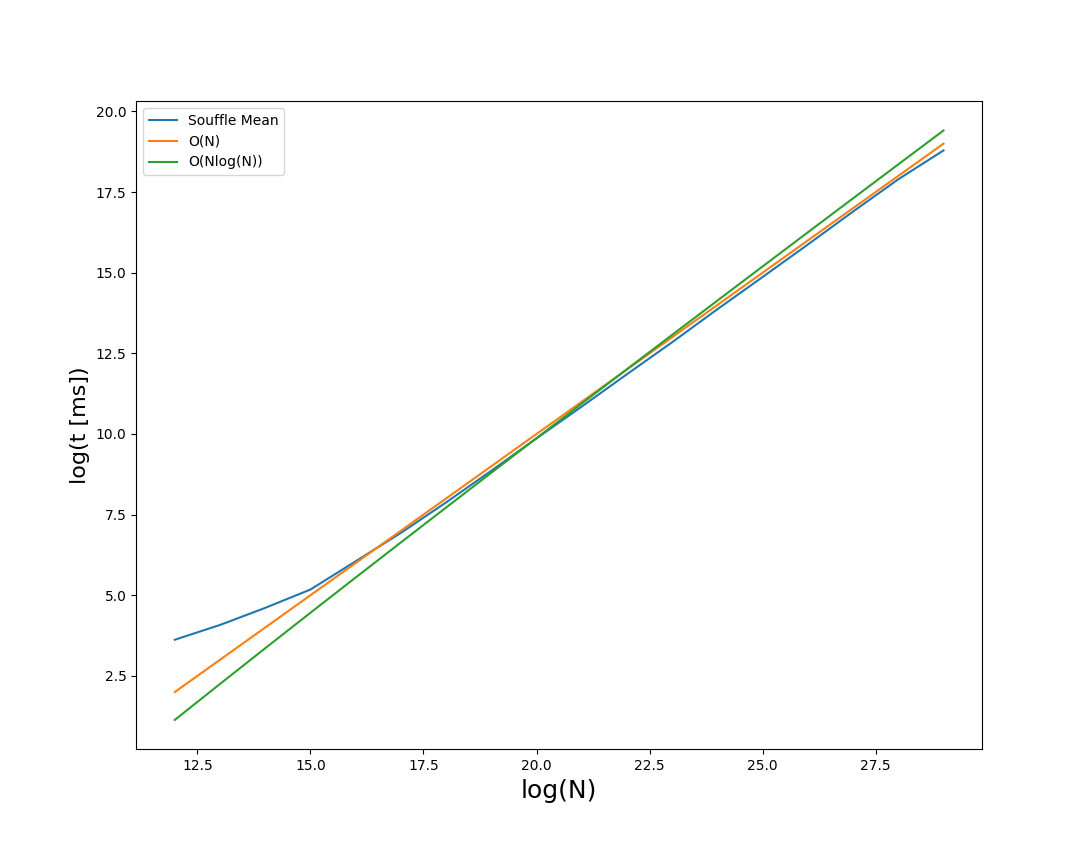
\includegraphics[scale=0.35]{img/souffleloglog.png}
%	%	\end{minipage}
%	%	\label{figure:natExperimental}
%	\caption{Nat Example, Souffle Evaluation (Semi-Naive)}
%\end{figure}
%\begin{figure}[!htb]
%	\centering
%	%	\hspace*{-25pt}
%	%	\begin{minipage}[b]{.5\textwidth}
%	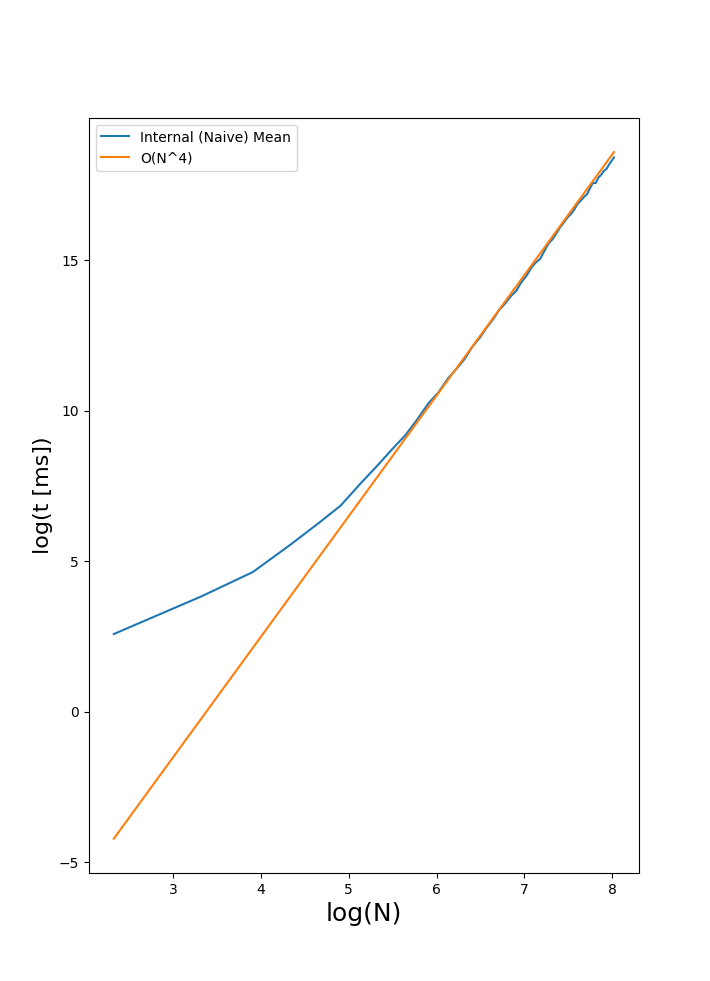
\includegraphics[width=1.0\linewidth]{img/ancestorInternal.png}
%	%\end{minipage}%
%	%	\hspace*{-40pt}
%	%	\begin{minipage}[b]{.5\textwidth}
%	%		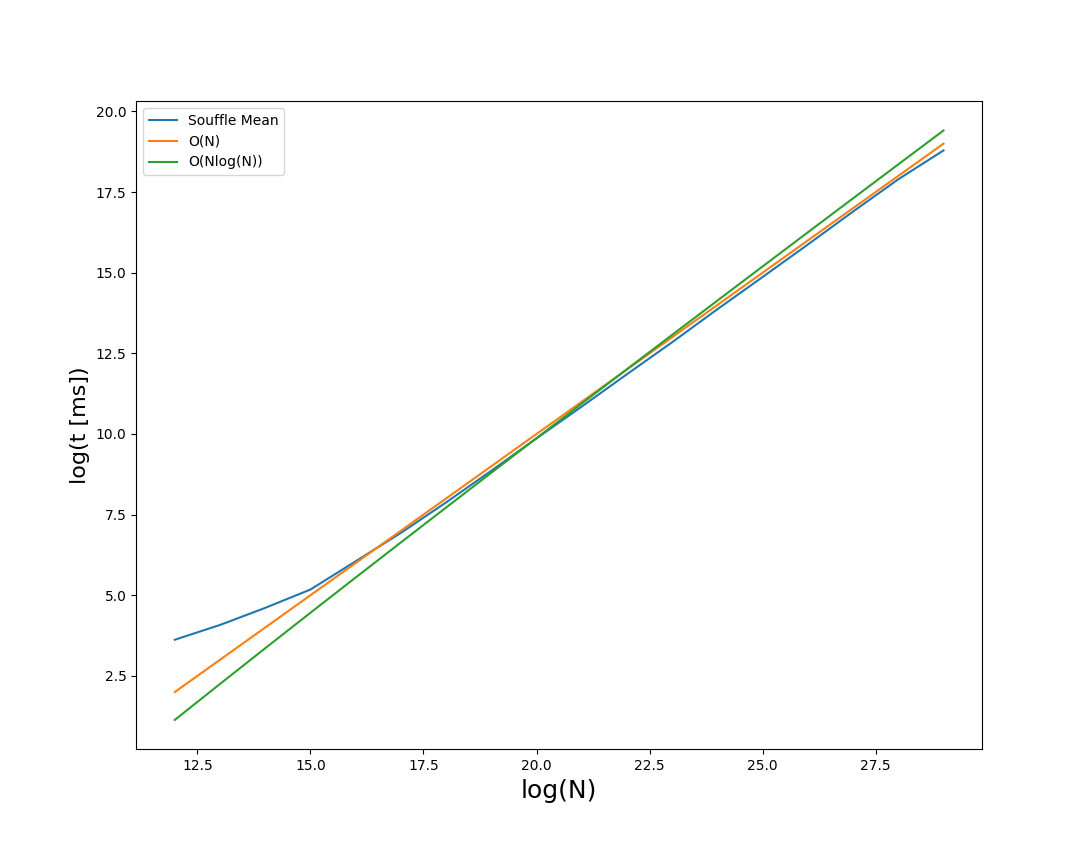
\includegraphics[scale=0.35]{img/souffleloglog.png}
%	%	\end{minipage}
%	%	\label{figure:natExperimental}
%	\caption{Nat Example, Souffle Evaluation (Semi-Naive)}
%\end{figure}
%\begin{figure}[!htb]
%	\centering
%	%	\hspace*{-25pt}
%	%	\begin{minipage}[b]{.5\textwidth}
%	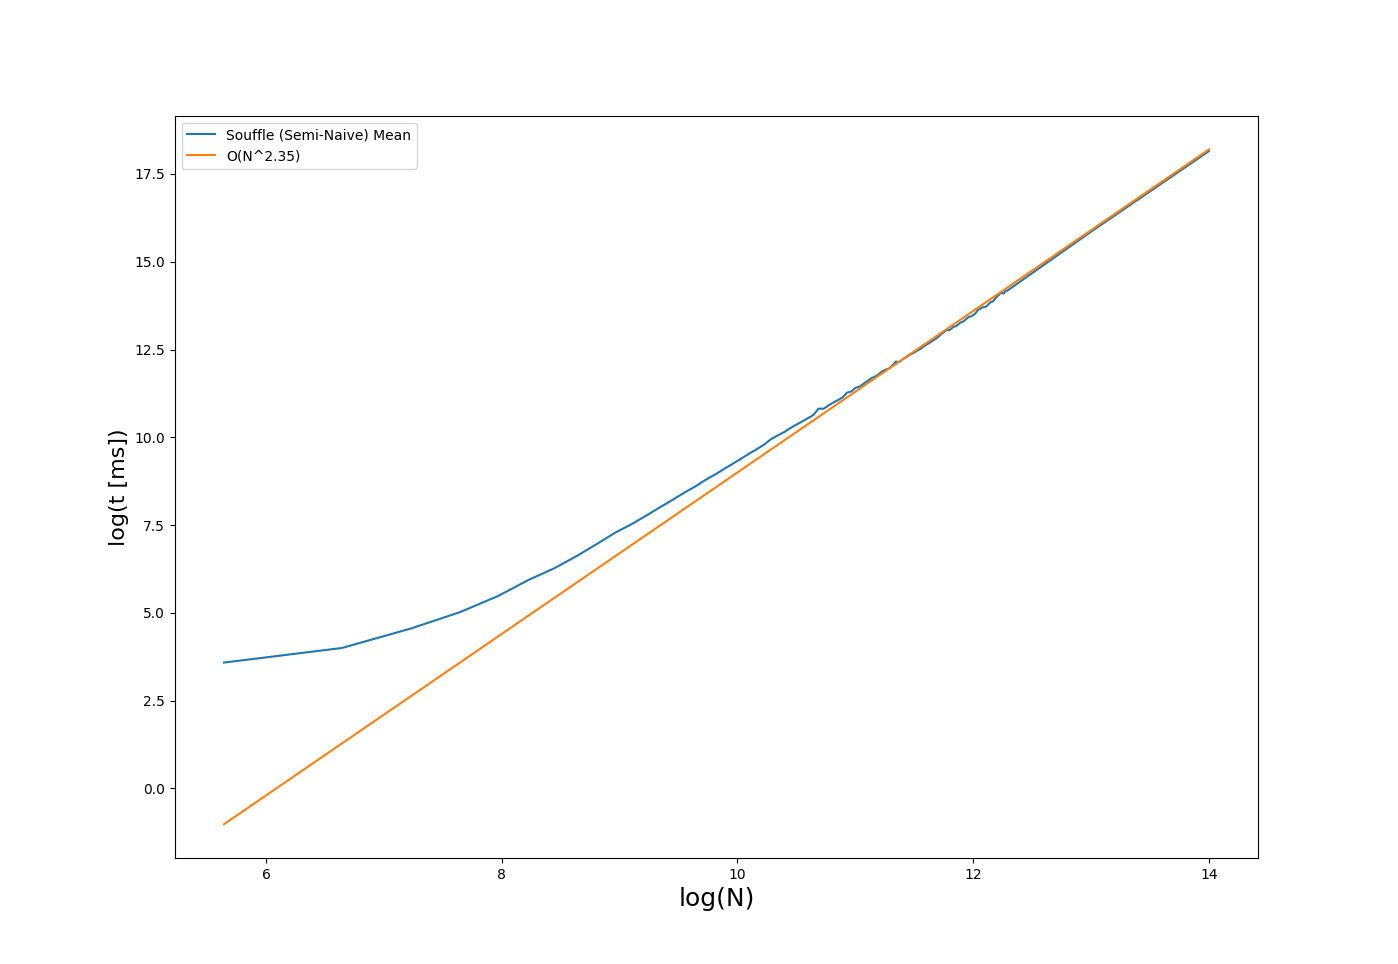
\includegraphics[width=1.0\linewidth]{img/ancestorSouffle.png}
%	%\end{minipage}%
%	%	\hspace*{-40pt}
%	%	\begin{minipage}[b]{.5\textwidth}
%	%		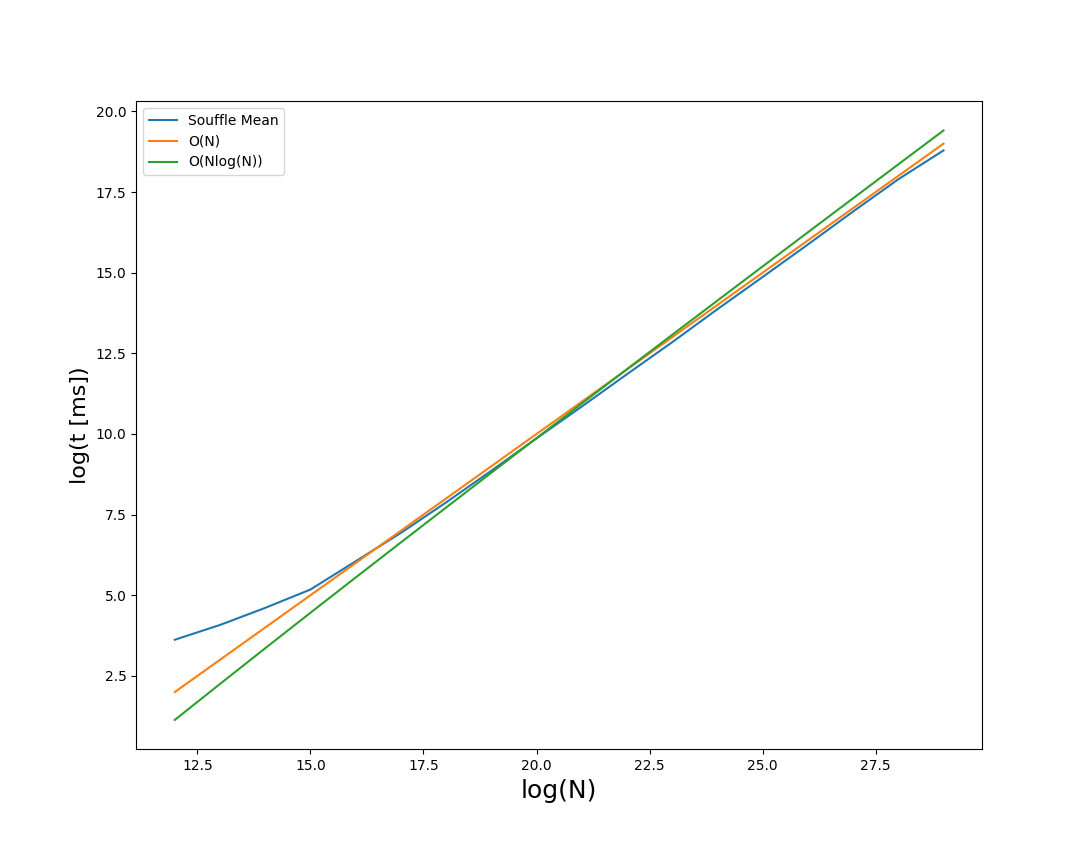
\includegraphics[scale=0.35]{img/souffleloglog.png}
%	%	\end{minipage}
%	%	\label{figure:natExperimental}
%	\caption{Nat Example, Souffle Evaluation (Semi-Naive)}
%\end{figure}
%
%
%%\begin{figure*}[!t]
%%	\hspace*{-70pt}
%%	\begin{minipage}[b]{.5\textwidth}
%%		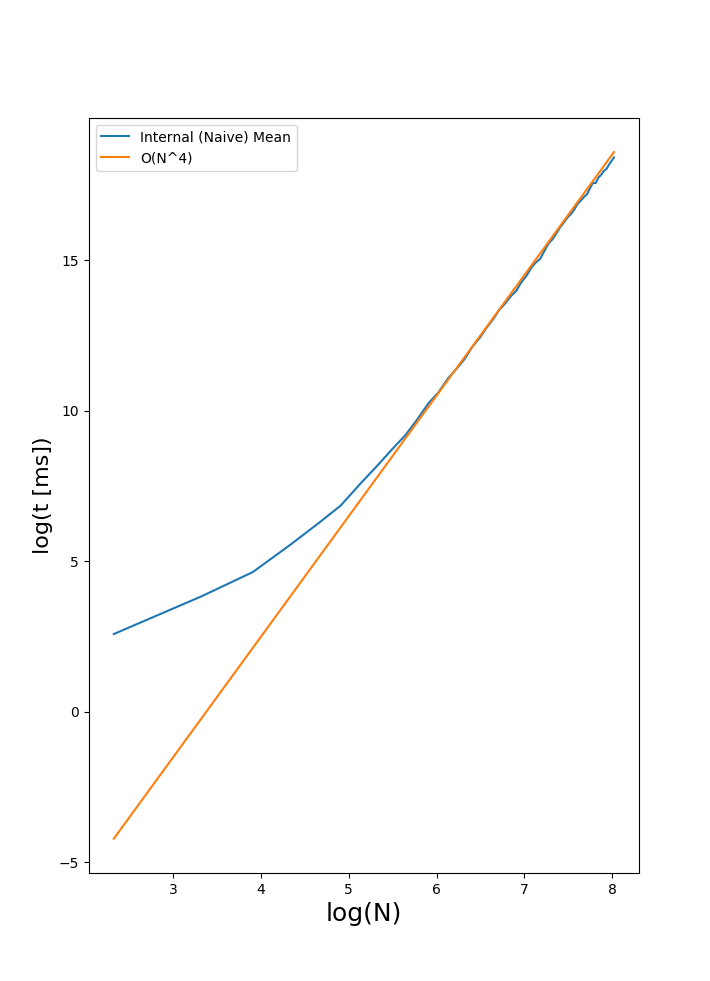
\includegraphics[scale=0.345]{img/ancestorInternal.png}
%%	\end{minipage}%
%%	\hspace*{-70pt}
%%	\begin{minipage}[b]{.5\textwidth}
%%		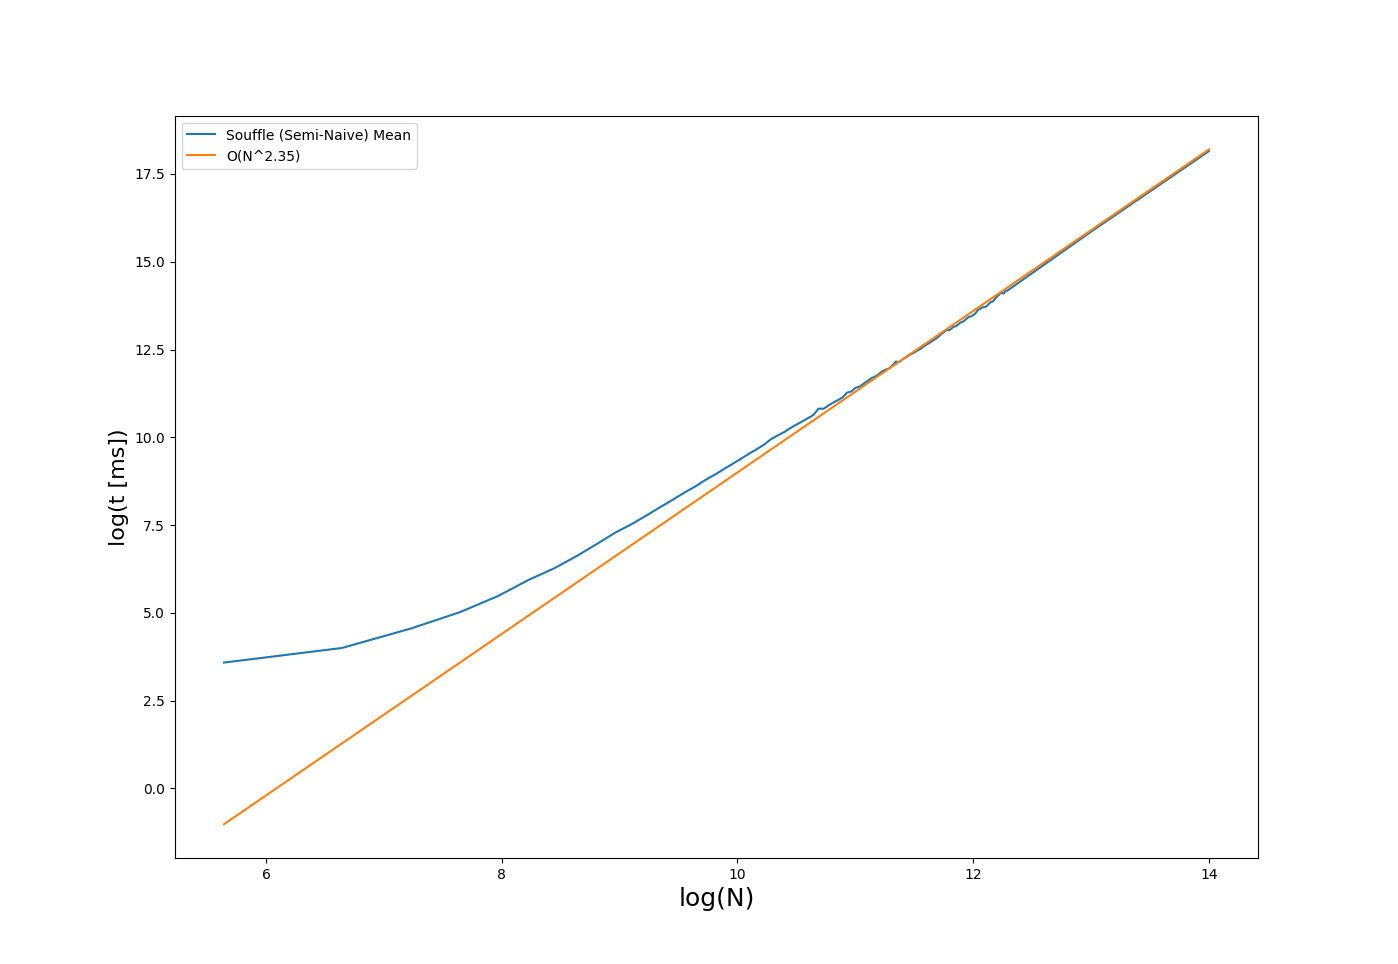
\includegraphics[scale=0.35]{img/ancestorSouffle.png}
%%	\end{minipage}
%%	\label{figure:ancestorExperimental}
%%	\caption{Ancestor Example, \textbf{Left: } Internal (Naive), \textbf{Right: } Souffle (Optimized Semi-Naive)}
%%\end{figure*}
\end{document}